%!TEX root = main.tex

\section{Reparameterizing the Acceptance-Rejection Sampler}\label{sec:method}

%\begin{figure*}[t]
%  \centering
%  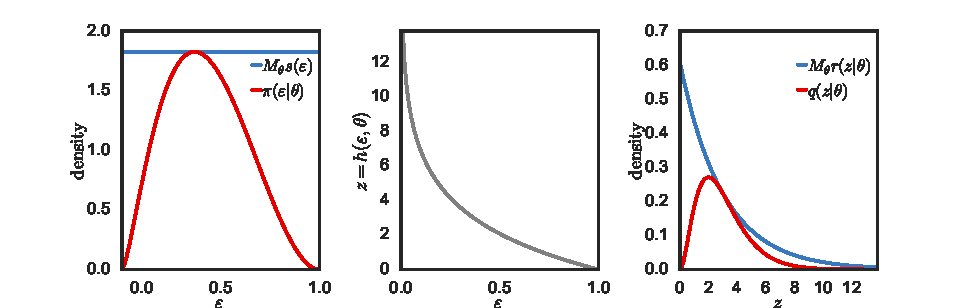
\includegraphics[width=6.5in]{dummy_gamma} 
%  \caption{Example of a reparameterized rejection sampler for~${q(z \g
%      \theta)= \gam(\theta,1)}$, shown here with~${\theta = 3}$.
%    For illustration purposes, we use an
%    inefficient exponential proposal distribution,~$r(z \g \theta) =
%    \expon(\theta^{-1})$, which is valid for~${\theta \geq 1}$.
%    The exponential proposal
%    distribution is reparameterized with the
%    transformation,~${h(\epsilon, \theta) = -\theta \log \varepsilon
%    }$, for~${\varepsilon \sim \uni(0,1)}$.  The marginal density of
%    the accepted values of~$\varepsilon$ (integrating out the
%    acceptance variables,~$u_{1:\tau}$) is given by~${\pi(\varepsilon \g
%      \theta)}$. We compute unbiased estimates of the gradient of the
%    ELBO~\eqref{eq:reparamgrad} via Monte Carlo, using
%    Algorithm~\ref{alg:rejectionsampling} to rejection
%    sample~${\varepsilon \sim \pi(\varepsilon \g \theta)}$. By reparameterizing
%    in terms of~$\varepsilon$, we obtain a low-variance estimator
%    of the gradient for challenging distributions.
%  }
%  \label{fig:dummy_gamma}
%\end{figure*}

\begin{figure*}[t]
  \centering
  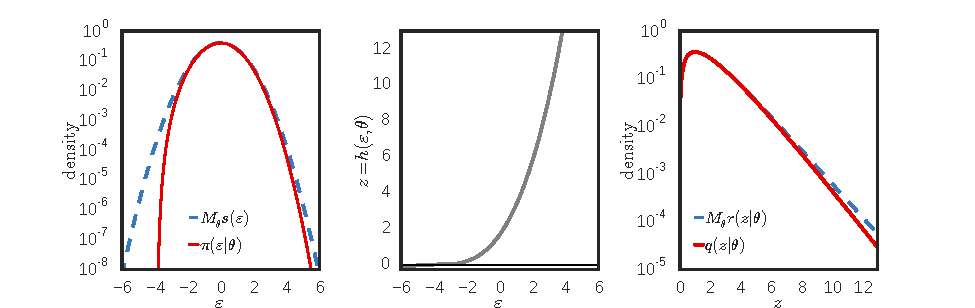
\includegraphics[width=6.5in]{real_gamma} 
  \caption{Example of a reparameterized rejection sampler for~${q(z \g
      \theta)= \gam(\theta,1)}$, shown here with~${\theta = 2}$.  We
    use the rejection sampling algorithm of \citet{Marsaglia:2000},
    which is based on a nonlinear transformation ${h(\varepsilon,
      \theta)}$ of a standard normal~${\varepsilon \sim \N(0,1)}$
    (c.f. Eq.~\ref{eq:marsaglia}), and has acceptance probability
    of~$0.98$ for~${\theta=2}$. The marginal density of the accepted
    value of~$\varepsilon$ (integrating out the acceptance
    variables,~$u_{1:i}$) is given by~${\pi(\varepsilon \g
      \theta)}$. We compute unbiased estimates of the gradient of the
    \gls{ELBO}~\eqref{eq:reparamgrad} via Monte Carlo, using
    Algorithm~\ref{alg:rejectionsampling} to rejection
    sample~${\varepsilon \sim \pi(\varepsilon \g \theta)}$. By
    reparameterizing in terms of~$\varepsilon$, we obtain a
    low-variance estimator of the gradient for challenging
    variational distributions.}
  \label{fig:real_gamma}
\end{figure*}


The basic idea behind reparameterization is to rewrite simulation from a complex distribution as a deterministic mapping of its parameters and a set of simpler random variables. We can view the rejection sampler as a complicated deterministic mapping of a (random) number of simple random variables such as uniforms and normals. This makes it tempting to take the standard reparameterization approach when we consider random variables generated by rejection samplers. However, this mapping is in general not continuous, and thus moving the derivative inside the expectation and using direct automatic differentiation would not necessarily give the correct answer.

Our insight is that we can overcome this problem by instead considering only the marginal over the accepted sample, analytically integrating out the accept-reject variable. Thus, the mapping comes from the proposal step. This is continuous under mild assumptions, enabling us to greatly extend the class of variational families amenable to reparameterization.

We first review rejection sampling and present the reparameterized rejection sampler. Next we show how to use it to calculate low-variance gradients of the \gls{ELBO}. Finally, we present the complete stochastic optimization for variational inference, \gls{RS-VI}.
%\cn{Notation, should we use $\pi(\eps\g \theta)$ to show that it in fact depends on theta?} 
% fjrr: yes! I already changed that (in Sec 3 only)

% ======================================================================
%   REJECTION SAMPLING
% ======================================================================
\subsection{Reparameterized Rejection Sampling}
Acceptance-Rejection sampling is a powerful way of simulating random variables from complex distributions whose inverse cumulative distribution functions are not available or are too expensive to evaluate \citep{devroye1986,robert2004monte}. We consider an alternative view of rejection sampling in which we explicitly make use of the reparameterization trick. This view of the rejection sampler enables our variational inference algorithm in Section~\ref{subsec:method}. 

To generate samples from a distribution $q(z\g\theta)$ using rejection sampling, we first sample from a \emph{proposal distribution} $r(z\g \theta)$ such that $q(z\g \theta) \leq M_\theta r(z\g \theta)$ for some $M_\theta <\infty$. In our version of the rejection sampler, we assume that the proposal distribution is reparameterizable, \ie, that generating $z\sim r(z\g \theta)$ is equivalent to generating $\eps \sim s(\eps)$ (where $s(\eps)$ does not depend on $\theta$) and then setting $z=h(\eps,\theta)$ for a differentiable function $h(\eps,\theta)$. We then accept the sample with probability $\min\left\{1, \frac{q\left(h(\eps,\theta)\g \theta\right)}{M_\theta r\left(h(\eps,\theta) \g \theta\right)}\right\}$; otherwise, we reject the sample and repeat the process. We illustrate this in Figure~\ref{fig:real_gamma} and provide a summary of the method in Algorithm~\ref{alg:rejectionsampling}, where we consider the output to be the (accepted) variable $\eps$, instead of $z$.

%To generate samples from $q(z\g \theta)$ we make use of a proposal distribution $r(z\g \theta)$, such that $q(z\g \theta) \leq M_\theta r(z\g \theta)$ for a constant $M_\theta <\infty$. We assume that generating $z\sim r(z\g \theta)$ is equivalent to $z=h(\eps,\theta), ~\eps \sim s(\eps)$, \ie we assume that a reparameterization of the \emph{proposal distribution} is possible. Furthermore, note that $s(\eps)$ does not depend on the parameters $\theta$, and $h(\eps,\theta)$ is assumed differentiable in $\theta$. Most often $s(\eps)$ is a simple distribution that we have efficient ways to generate samples from, such as the uniform $\uni[0,1]$ or standard Normal $\N(0,1)$. We provide a summary of the method in Algorihm~\ref{alg:rejectionsampling} where we actually assume the output to be $\eps$, \ie the accepted $\eps$ for the accepted iteration $\tau$. This view of the rejection sampler, where the output is $\eps$, is a non-standard approach that will be key to allowing us to leverage the reparameterization trick in estimating the gradient of the \elbo.



%\begin{remark}
The ability to simulate from $r(z\g \theta)$ by a reparameterization through a differentiable $h(\eps,\theta)$ is not needed for the rejection sampler to be valid. However, this is indeed the case for the rejection sampler of many common distributions.
%\end{remark}

\begin{algorithm}[t]
\caption{Reparameterized Rejection Sampling}\label{alg:rejectionsampling}
\begin{algorithmic}[1]
\REQUIRE target $q(z\g \theta)$, proposal $r(z\g \theta)$, and constant $M_\theta$, with $q(z\g \theta) \leq M_\theta r(z\g \theta)$ 
\ENSURE $\eps$ such that $h(\eps,\theta) \sim q(z\g \theta)$
\STATE $i \gets 0$
\REPEAT 
\STATE $i \gets i +1 $
\STATE Propose $\eps_i \sim s(\eps)$
\STATE Simulate $u_i \sim \uni[0,1]$
\UNTIL $u_i < \frac{q\left(h(\eps_i,\theta)\g \theta\right)}{M_\theta r\left(h(\eps_i,\theta) \g \theta\right)}$
\RETURN $\eps_i$
\end{algorithmic}
\end{algorithm}



% ======================================================================
%
% ======================================================================
\subsection{The Reparameterized Rejection Sampler in Variational Inference}
\label{subsec:method}

We now use reparameterized rejection sampling to develop a novel Monte Carlo estimator of the gradient of the \gls{ELBO}. We first rewrite the \gls{ELBO} in \eqref{eq:elbo} as an expectation in terms of the transformed variable $\eps$,
\begin{align}
\begin{split}
&\Lo(\theta) = \E_{q(z\g \theta)}\left[f(z)\right] + \Ent[q(z\g \theta)] \\
&\quad\quad=\E_{\pi(\eps\g\theta)}\left[f\left(h(\eps,\theta)\right)\right] + \Ent[q(z\g \theta)].
\end{split}
\label{eq:ReparamExp}
\end{align}
In this expectation, $\pi(\eps\g\theta)$ is the distribution of the \emph{accepted sample} $\eps$ in Algorithm~\ref{alg:rejectionsampling}. We construct it by marginalizing over the auxiliary uniform variable $u$,
\begin{align}
\pi(\eps\g\theta) &= \int \pi(\eps,u\g\theta) \myd u \nonumber\\
&= \int M_\theta s(\eps) 
%\mathbbm{1}
\mathds{1}
\left[0 < u < \frac{q\left(h(\eps,\theta)\g \theta\right)}{M_\theta r\left(h(\eps,\theta)\g \theta\right)}\right] \myd u \nonumber\\
&= s(\eps) \frac{q\left(h(\eps,\theta)\g \theta\right)}{r\left(h(\eps,\theta)\g \theta\right)},
\label{eq:distrejection}
\end{align}
where $\mathds{1}[x \in A]$ is the indicator function, and recall that $M_\theta$ is a constant used in the rejection sampler. %which takes value $1$ if $x \in A$ and $0$ otherwise. 
This can be seen by the algorithmic definition of the rejection sampler, where we propose values $\eps \sim s(\eps)$ and $u \sim \uni[0,1]$ until acceptance, \ie, until $u < \frac{q\left(h(\eps,\theta)\g \theta\right)}{M_\theta r\left(h(\eps,\theta) \g \theta\right)}$. Eq.~\ref{eq:ReparamExp} follows intuitively, but we formalize it in Proposition~\ref{thm:reparam}.



%where $\pi(\eps)$ is the distribution for $\eps$ implicitly defined by Algorithm~\ref{alg:rejectionsampling}. The equality inuitively follows because ${z=h(\eps,\theta)}$ for $\eps \sim \pi(\eps)$ implies that $z\sim q(z\g \theta)$ by standard properties of the rejection sampler, \ie it is a form of reparameterization. Below we show more formally that this is true. We can find the distribution $\pi(\eps)$ by noting that it is in fact the marginal over the joint distribution of $\eps,u$, \ie accepted proposal and the auxiliary accept--reject uniform, \ie%The reason why we choose to include $u$ will be made clear below. The joint distribution over $\eps$ and $u$ is given by

%The reparameterization in \eqref{eq:ReparamExp} and the connection with $\pi(\eps\g\theta)$ in \eqref{eq:distrejection} is key to our method so we formalize it in Theorem~\ref{thm:reparam}.

\begin{proposition}
\label{thm:reparam}
Let $f$ be any measurable function, and $\eps \sim \pi(\eps\g\theta)$, defined by \eqref{eq:distrejection} (and implicitly by Algorithm~\ref{alg:rejectionsampling}). Then
\begin{align*}
&\E_{\pi(\eps\g\theta)}\left[f\left(h(\eps,\theta)\right)\right] = \int f(z) q(z\g \theta) \myd z.
\end{align*}
\end{proposition}
\begin{proof}
Using the definition of $\pi(\eps\g\theta)$,
\begin{align*}
&\E_{\pi(\eps\g\theta)}\left[f\left(h(\eps,\theta)\right)\right] 
%&=\int f\left(h(\eps,\theta)\right) M_\theta s(\eps) \int \mathbbm{1}_{0 < u < \frac{q\left(h(\eps,\theta)\g \theta\right)}{M_\theta r\left(h(\eps,\theta)\g \theta\right)}} \myd u \myd \eps \\
%&= \int f\left(h(\eps,\theta)\right) M_\theta s(\eps) \int_0^{\frac{q\left(h(\eps,\theta)\g \theta\right)}{M_\theta r\left(h(\eps,\theta)\g \theta\right)}} 1 \myd u \myd \eps \\
=\int f\left(h(\eps,\theta)\right) s(\eps) \frac{q\left(h(\eps,\theta)\g \theta\right)}{ r\left(h(\eps,\theta)\g \theta\right)}  \myd \eps \\
&= \int  f(z) r(z\g \theta) \frac{q(z\g \theta)}{r(z\g \theta)} \myd z = \int f(z) q(z\g \theta) \myd z,
\end{align*}
where the second to last equality follows because ${h(\eps,\theta), \eps \sim s(\eps)}$ is a reparameterization of $r(z\g \theta)$.% \cn{Cite Law of the Unconcious Statistician here?}
\end{proof}
%This lets us write \eqref{eq:elbo}, the \elbo, as an expectation with respect to the output of the rejection sampler
%\begin{align*}
%&\E_{\pi(\eps,u)}\left[f\left(h(\eps,\theta)\right)\right] = \\
%&=\int M_\theta s_\eps(\eps) f\left(h(\eps,\theta)\right) \int_0^{\frac{q_\theta\left(h(\eps,\theta)\right)}{M_\theta r_\theta\left(h(\eps,\theta)\right)}} 1 \myd u \myd \eps\\
%&=\int M_\theta s_\eps(\eps) f\left(h(\eps,\theta)\right) \frac{q_\theta\left(h(\eps,\theta)\right)}{M_\theta r_\theta\left(h(\eps,\theta)\right)} \myd \eps\\
%&= \int q_\theta(z) f(z) \myd z,
%\end{align*}
%where the last equality follows because $h(\eps,\theta)$ is a reparameterization of $r_\theta(z)$.
We can now compute the gradient of $\E_{q(z\g \theta)}[f(z)]$ based on Eq.~\ref{eq:ReparamExp},
\begin{align}
\begin{split}
&\grad_\theta \E_{q(z\g \theta)}[f(z)] = \grad_\theta \E_{\pi(\eps\g\theta)}[f(h(\eps,\theta))] \\
%&= \int s(\eps) \grad_\theta \left( f\left(h(\eps,\theta)\right)  \frac{q\left(h(\eps,\theta)\g \theta\right)}{r\left(h(\eps,\theta)\g \theta\right)}  \right) \myd \eps\\
%&= \int s(\eps)  \frac{q\left(h(\eps,\theta)\g \theta\right)}{r\left(h(\eps,\theta)\g \theta\right)}  \grad_\theta f\left(h(\eps,\theta)\right)  \myd \eps\\
%&+ \int s(\eps) f\left(h(\eps,\theta)\right)  \grad_\theta \left( \frac{q\left(h(\eps,\theta)\g \theta\right)}{r\left(h(\eps,\theta)\g \theta\right)} \right) \myd \eps\\
&= \underbrace{\E_{\pi(\eps\g\theta)}[\grad_\theta f(h(\eps,\theta))]}_{\defeq g_{\text{rep}}}+ \\
&\quad + \underbrace{\E_{\pi(\eps\g\theta)}\left[ f(h(\eps,\theta)) \grad_\theta  \log \frac{q(h(\eps,\theta)\g \theta)}{r(h(\eps,\theta)\g \theta)} \right]}_{\defeq g_{\text{cor}}},
\end{split}\label{eq:graddef}
\end{align}
where we have used the log-derivative trick and rewritten the integrals as expectations with respect to $\pi(\eps\g\theta)$ (see the supplement for all details.) We define $g_{\text{rep}}$ as the reparameterization term, which takes advantage of gradients with respect to the model and its latent variables; we define $g_{\text{cor}}$ as a correction term that accounts for \emph{not} using $r(z\g \theta) \equiv q(z\g \theta)$.

%and the fact that we can write 
%\begin{align*}
%\frac{q\left(h(\eps,\theta)\g \theta\right)}{r\left(h(\eps,\theta)\g \theta\right)} = M_\theta \int_0^{\frac{q\left(h(\eps,\theta)\g \theta\right)}{M_\theta r\left(h(\eps,\theta)\g \theta\right)}} 1\myd u,
%\end{align*}
%as well as identifying the resulting expressions as expectations with respect to the joint distribution of $\eps$ and $u$.

%\cn{Not super satisfied with this part below:}

Using \eqref{eq:graddef}, the gradient of the \gls{ELBO} in \eqref{eq:elbo} can be written as
\begin{align}
\begin{split}
&\grad_\theta \Lo(\theta)  = g_{\text{rep}}+ g_{\text{cor}}+\grad_\theta \Ent[q(z\g\theta)],
\end{split}
\label{eq:reparamgrad}
\end{align}
and thus we can build an unbiased one-sample Monte Carlo estimator $\hat g \approx \grad_\theta \Lo(\theta)$ as
\begin{align}
\begin{split}
&\hat g  \eqdef \hat g_{\text{rep}} + \hat g_{\text{cor}}+\grad_\theta \Ent[q(z\g\theta)], \\
& \hat g_{\text{rep}} = \grad_z f(z)\big|_{z=h(\eps,\theta)} \grad_\theta h(\eps,\theta) \\
& \hat g_{\text{cor}} = f(h(\eps,\theta)) \grad_\theta  \log \frac{q(h(\eps,\theta)\g \theta)}{r(h(\eps,\theta)\g \theta)},
\end{split}
\label{eq:reparamgrad2}
\end{align}
where $\eps$ is a sample generated using Algorithm~\ref{alg:rejectionsampling}. Of course, one could generate more samples of $\eps$ and average, but we have found a single sample to suffice in practice.
%We can see that the first term, $g_{\text{rep}}$, a reparameterization term taking advantage of gradients with respect to the model and its latent variables. The second term, $g_{\text{cor}}$, can be seen as a kind of correction term for not using $r_\theta(z) = q_\theta(z)$. 
%However, if the acceptance rate in the rejection sampler is high the second term is typically very low. 

%\cn{Actually the following might only hold for $h$ invertible, it might however possible to generalize...}

%\fr{Is this necessary?} \cn{I think it is useful for practical considerations, and i ref it in Examples}

Note if $h(\eps,\theta)$ is invertible in $\eps$ then we can simplify the evaluation of the gradient of the log-ratio in $g_{\text{cor}}$,
\begin{align}
&\grad_\theta  \log \frac{q(h(\eps,\theta)\g \theta)}{r(h(\eps,\theta)\g \theta)}  = \nonumber\\
&\quad\quad\quad\grad_\theta  \log q(h(\eps,\theta)\g \theta) + \grad_\theta \log \left| \frac{d h}{d\eps}(\eps,\theta) \right| .\label{eq:gradQRcorr}
\end{align}
See the supplementary material for details.

%\begin{remark}
Alternatively, we could rewrite the gradient as an expectation with respect to $s(\eps)$ (this is an intermediate step in the derivation shown in the supplement),
\begin{align}
&\grad_\theta \E_{q(z\g \theta)}[f(z)] = \E_{s(\eps)}\left[ \frac{q\left(h(\eps,\theta)\g \theta\right)}{r\left(h(\eps,\theta)\g \theta\right)}  \grad_\theta f\left(h(\eps,\theta)\right)  \right]+ \nonumber\\
&+\E_{s(\eps)}\left[ \frac{q\left(h(\eps,\theta)\g \theta\right)}{r\left(h(\eps,\theta)\g \theta\right)}   f\left(h(\eps,\theta)\right) \grad_\theta \log  \frac{q\left(h(\eps,\theta)\g \theta\right)}{r\left(h(\eps,\theta)\g \theta\right)}  \right],\nonumber
\end{align}
and build an importance sampling-based Monte Carlo estimator, in which the importance weights would be $q\left(h(\eps,\theta)\g \theta\right) / r\left(h(\eps,\theta)\g \theta\right)$.
However, we would expect this approach to be beneficial for low-dimensional problems only, since for high-dimensional $z$ the variance of the importance weights would be too high.


\begin{algorithm}
\caption{Rejection Sampling Variational Inference}\label{alg:svi}
\begin{algorithmic}[1]
\REQUIRE Data $x$, model $p(x,z)$, variational family $q(z\g \theta)$
\ENSURE Variational parameters $\theta^*$
\REPEAT
\STATE Run Algorithm~\ref{alg:rejectionsampling} for $\theta^n$ to obtain a sample $\eps$
\STATE Estimate the gradient $\hat g^n$ at $\theta = \theta^n$ (Eq.~\ref{eq:reparamgrad2})
\STATE Calculate the stepsize $\rho^n$ (Eq.~\ref{eq:stepsize})
\STATE Update $\theta^{n+1} = \theta^n + \rho^n \hat{g}^n$
\UNTIL \textbf{convergence}
\end{algorithmic}
\end{algorithm}

% ======================================================================
%   COMPLETE ALGORITHM
% ======================================================================
\subsection{Full Algorithm}
We now describe the full variational algorithm based on reparameterizing the rejection sampler. In Section~\ref{sec:examples} we give concrete examples of how to reparameterize common variational families.

We make use of Eq.~\ref{eq:reparamgrad} to obtain a Monte Carlo estimator of the gradient of the \gls{ELBO}. We use this estimate to take stochastic gradient steps. We use the step-size sequence $\rho^n$ proposed by \citet{Kucukelbir2016} (also used by \citet{RuizTB2016}), which combines \textsc{rmsprop} \citep{Tieleman2012} and Adagrad \citep{Duchi2011}. It is
\begin{align}
\begin{split}
\rho^n &= \eta \cdot n^{-1/2 + \delta} \cdot \left(1 + \sqrt{s^n}\right)^{-1},\\
s^n &= t \left( \hat{g}^n \right)^2 + (1-t) s^{n-1},
\label{eq:stepsize}
\end{split}
\end{align}
%To arrive at a complete algorithm for stochastic optimization of \eqref{eq:elbo}, the \elbo, we require a step-size sequence $\rho^n$ that ensures convergence. We propose to make use of the one , which 
where $n$ is the iteration number. We set $\delta = 10^{-16}$ and $t=0.1$, and we try different values for $\eta$. (When~$\theta$ is a vector, the operations above are element-wise.)

We summarize the full method in Algorithm~\ref{alg:svi}. We refer to our method as \gls{RS-VI}. %\cn{more awesome name?}Note that we can handle larger datasets by combining subsampling as in stochastic variational inference \citep{Hoffman2013} with Algorithm~\ref{alg:svi}. This is a type of doubly stochastic variational inference algorithm \citep{Titsias2014_doubly}. 
